\documentclass[conference]{IEEEtran}
\usepackage{bm}
\usepackage{cite}
\usepackage{ragged2e}
\usepackage{graphicx}
\usepackage{amsmath}
\usepackage{amssymb}
\usepackage{amsthm}
\usepackage{algorithm}
\usepackage{algpseudocode}
\usepackage{enumitem}
\usepackage{etoolbox}
\usepackage{mathrsfs}
\usepackage{subfig}
\usepackage{array}
\usepackage{cases}
\usepackage{dsfont}
\usepackage{optidef}
\usepackage{cleveref}

\allowdisplaybreaks
\newtheorem{theorem}{Theorem}
\newtheorem{lemma}{Lemma}
\newtheorem{definition}{Definition}
\setlength{\columnsep}{0.21in}
\makeatletter
\newcommand\fs@betterruled{%
  \def\@fs@cfont{\bfseries}\let\@fs@capt\floatc@ruled
  \def\@fs@pre{\vspace*{0.03in}\hrule height.8pt depth0pt \kern2pt}%
  \def\@fs@post{\kern2pt\hrule\relax}%
  \def\@fs@mid{\kern2pt\hrule\kern2pt}%
  \let\@fs@iftopcapt\iftrue}
\floatstyle{betterruled}
\restylefloat{algorithm}
\makeatother
\renewcommand{\arraystretch}{1.2}
\begin{document}
\title{Final Report for Wireless Mobile Network}
\author{\IEEEauthorblockN{Chia-Hung Lin, Chun-Yen Lee, Lu-Yo Kuo}
\IEEEauthorblockA{
Department of Electrical Engineering, National Taiwan University \\
b06504016@ntu.edu.tw, b06203017@ntu.edu.tw, b06502153@ntu.edu.tw
}}
\maketitle
\begin{abstract}
In this final project, we mainly simulate the D2D system and multicast system.
\end{abstract}

\section{Introduction}
To be added
\section{HW5}
\subsection{System Model}
The system is about Device to Device (D2D) systems. The distance between receive and transmission pair is fixed to $100m$. Both transmission user equipment (UE) and receive UE are in the central cell. There are $75$ UE pairs in the system.
\begin{figure}[htbp]
    \centering
    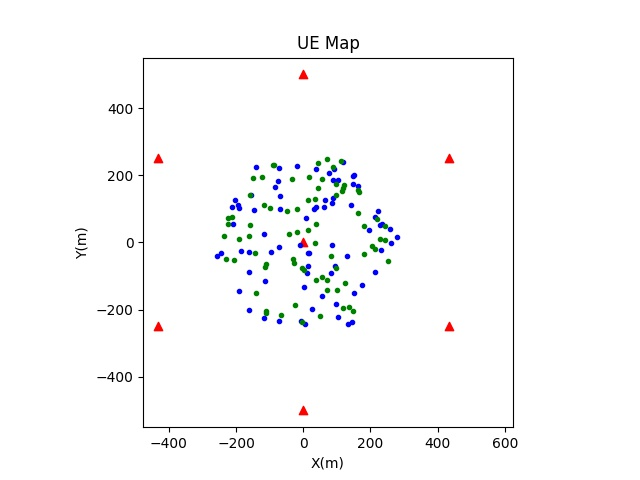
\includegraphics[width=0.45\textwidth]{fig1_1.jpg}
    \caption{The simulated map for UEs}
    \label{fig:ue_map}
\end{figure}


In \Cref{fig:ue_map}, the green point indicates the receive UE, and the blue point indicates the transmission UE. The red triangle indicates the base stations in the system.
\subsection{Basic D2D Topology Simulation}
\subsubsection{Simulation Parameters}
In the system, the bandwidth is $10$MHz, the temperature is $27^\circ$C, the power of the base stations is $23$dBm, the power of UEs in $0$dBm, the antenna gain of receive and transmit is both $0$dB. The UE height is $1.5$m, and the base station height is $51.5$m. The path loss model is Two-ray-ground model, which can be written as
\begin{equation}\label{eqn:two_ray}
    g(d) = P_t \times \dfrac{Gh_t^2h_r^2}{d^4}
\end{equation}
where $P_t$ is the transmit power, and $G$ is the total gain, $h_t$ and $h_r$ are height of transmit and receive antennas respectively.
\subsubsection{PMF for Uplink SINR}
In the uplink scenario, as shown in \Cref{fig:uplink_sinr}, the SINR of the uplink signal is between $60$ to $100$ dB, which is very large. This can be explained by the assumption that there is no interference in the uplink transmission.
\begin{figure}[htbp]
    \centering
    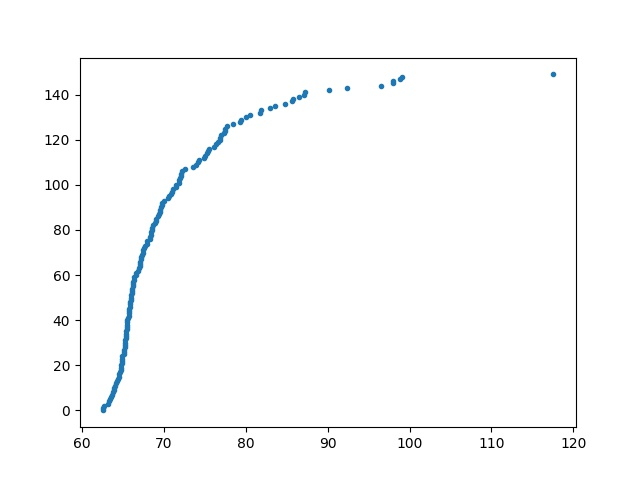
\includegraphics[width=0.45\textwidth]{fig1_2_a.jpg}
    \caption{PMF for Uplink SINR}
    \label{fig:uplink_sinr}
\end{figure}

\subsubsection{PMF for Downlink SINR}
In the downlink scenario, as shown in \Cref{fig:downlink_sinr}, the SINR of the downlink signal is between $0$ to $50$ dB.
\begin{figure}[htbp]
    \centering
    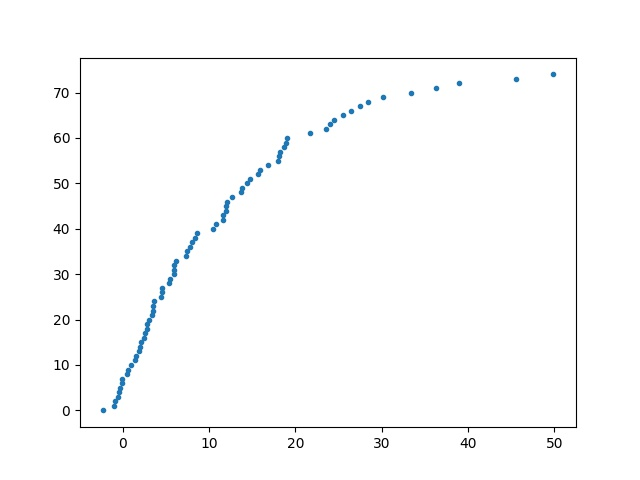
\includegraphics[width=0.45\textwidth]{fig1_2_b.jpg}
    \caption{PMF for Downlink SINR}
    \label{fig:downlink_sinr}
\end{figure}
Although the power of the downlink is from the base station, the SINR is smaller than the uplink signal. This difference is mainly caused by the different presumption of the uplink and downlink transmission signal, where the uplink signal is hypothesized to be interference-free, and the downlink signal is assumed to be interference by the signal from other base station.
\subsubsection{Total Throughput of the Downlink transmission}
By the simulation, the total throughput is approximately $2.43$ Gbps.
\subsubsection{PMF of the D2D SINR}
In D2D system, as shown in \Cref{fig:d2d_sinr}, the SINR of the D2D signal is mostly between $-60$ to $-10$ dB.

\begin{figure}[htbp]
    \centering
    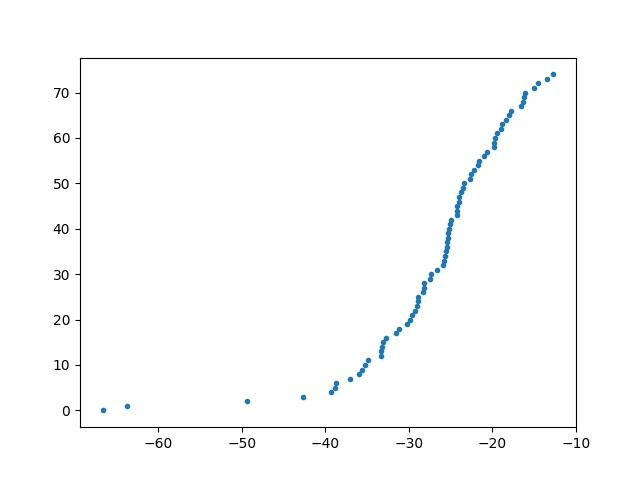
\includegraphics[width=0.45\textwidth]{fig1_4.jpg}
    \caption{PMF for D2D SINR}
    \label{fig:d2d_sinr}
\end{figure}
The huge gap of SINR between D2D systems and up/down link systems is caused by various reasons. Mostly, it is caused by the interference signal of other D2D pairs.
\subsubsection{Total Throughput of the D2D system}
By the simulation, the total throughput is approximately $9.98$ Mbps.
\subsubsection{Total Throughput with different number of D2D pairs}
As seen in \Cref{fig:d2d_num}, when the number of D2D pairs increases, the total through put is likely to decline.

\begin{figure}[htbp]
    \centering
    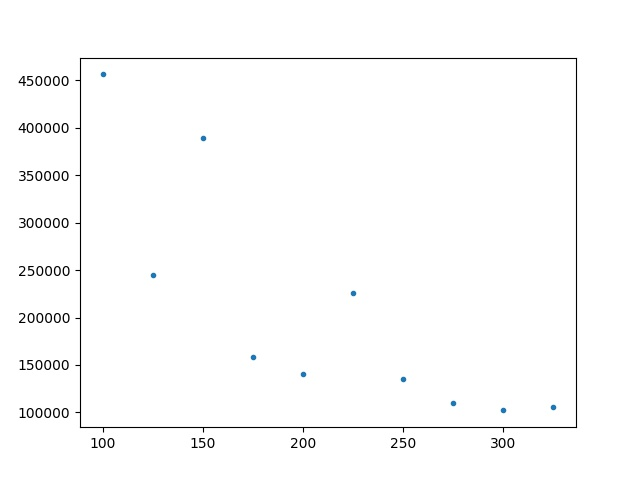
\includegraphics[width=0.45\textwidth]{fig1_6.jpg}
    \caption{Total Throughput vs. Number of D2D Pair}
    \label{fig:d2d_num}
\end{figure}
 This phenomenon is generated by the interference of other UEs. If the number of pairs increases, the distance between the receive UE and other transmit UE is very likely to be close, hence the increase of interference. However, the curve is not strictly decreasing for several reasons, the fluctuation is mainly caused by the difference of distance between the D2D pairs.
\subsection{Traffic in D2D Simulation}

\subsubsection{Bit Loss Probability in UL/DL systems}
In UL/DL systems, the SINR is huge in contrast to the D2D systems. In the simulation, the data rate is between $100$kbps to $2$Mbps. In \Cref{fig:uplink_sinr}, the median SINR is about 70 dB. By the Shannon Capacity
\begin{equation} \label{eqn:shannon}
    C = BW \times log_2(1 + SINR)
\end{equation}
the rate is approximately $10^6 \times log_2(1+ 10 \times 10^7) \approx 26$Mbps, which is far faster than the data rate. Therefore, we added a new high data rate of $200$Mbps to test whether the high data rate causes bit loss. Same as expected, the bit loss probability is about $80\%$.
\begin{figure}[htbp]
    \centering
    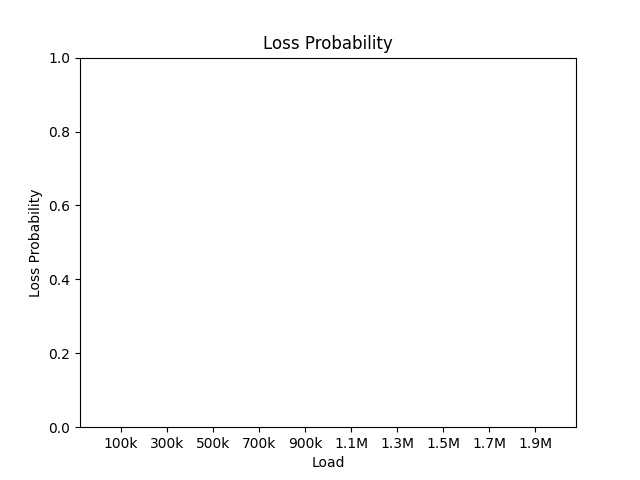
\includegraphics[width=0.45\textwidth]{fig2_1.jpg}
    \caption{Bit Loss Probability of various data rate in UL/DL systems}
    \label{fig:bit_uldl}
\end{figure}
\subsubsection{Bit Loss Probability in D2D system}
In \Cref{fig:d2d_sinr}, we have discovered that in D2D systems, the median of SINR is approximately $-25$dB. By \Cref{eqn:shannon}, the transmit rate of the D2D system is about $10^6 \times log_2(1+ 10 \times 10^{-2.5}) \approx 4.5$kbps
\begin{figure}[htbp]
    \centering
    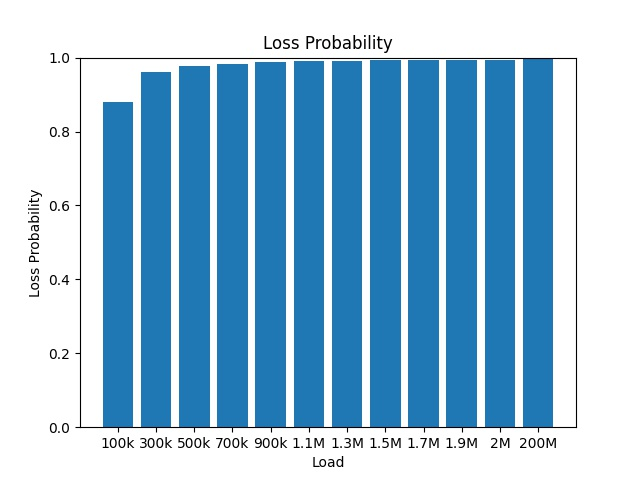
\includegraphics[width=0.45\textwidth]{fig2_2.jpg}
    \caption{Bit Loss Probability of various data rate in D2D systems}
    \label{fig:bit_d2d}
\end{figure}
\section{HW6}

\subsection{System Model}
The system is about multicast systems. The number of mobile stations (MS) in each inner base station (BS) is randomly selected from uniform distribution between $[5, 15]$. The base stations will transmit the same data to these mobile stations simultaneously. There are two schemes of multicast. One is Point to Multipoint (PTM), and the other is Single Frequency Network (SFN).
\begin{figure}[htbp]
    \centering
    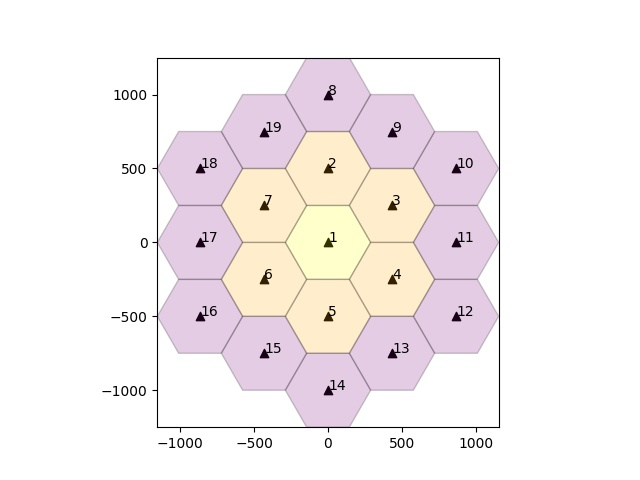
\includegraphics[width=0.45\textwidth]{Cell_ID.jpg}
    \caption{The simulated map for base stations}
    \label{fig:bs_map}
\end{figure}
In \Cref{fig:bs_map}, the orange part is the coverage of seven inner base stations (1-7), while the purple part is the coverage of outer base stations (8-19). We consider the problem that inner BSs multicast to the MSs in inner BSs.
\subsection{Simulation}

\section{Conclusion}
The conclusion goes here.
\end{document}
